Der Client ist entweder ein KI-Client, der von Software gesteuert ist oder ein Benutzer-Client, der von einem Menschen gesteuert wird. Deshalb gibt es eine extend-Relation von den beiden Akteuren 'KI-Client' und 'Benutzer-Client' zum abstrakten Client. \\
Nachdem der Client die Verbindung aufgebaut hat, muss die Verbindung von Client und Server gehalten werden, deshalb ist der Anwendungsfall 'Verbindung halten' mit einer include-Relation an den Anwendungsfall 'Verbindung initiieren' gebunden. \\
Die Dateien des Spiels müssen im JSON-Format über die Verbindung übertragen werden, deshalb die include-Relation vom Anwendungsfall 'Verbindung halten' zum Anwendungsfall 'JSON-Codierung'. \\
Falls die Verbindung abbricht, muss die Verbindung wieder aufgebaut werden, damit die Verbindung gehalten ist. Deshalb gibt es eine include-Relation vom Anwendungsfall 'Verbindung halten' zum Anwendungsfall 'Verbindung wieder aufbauen'. \\
Wenn der Client eine Verbindung zum Server initiiert, muss der Client dem Server übermitteln, ob es sich um einen KI-Client oder um einen von Menschen gesteuerten Client handelt. Deshalb gibt es eine include-Relation vom Anwendungsfall 'Verbindung initiieren' zum Anwendungsfall 'Registrieren des Client-Typs'. \\
Falls der Client während dem Halten der Verbindung die Anwortfrist nicht einhält, so soll der Server die Verbindung zum Client trennen. Deshalb gibt es eine bedingte extend-Relation vom Anwendungsfall 'Verbindung trennen' zum Anwendungsfall 'Verbindung halten'. \\


Anforderungsabdeckungen:\\

Verbindung initiieren

FA-C \ref{c-session} %FA-C 33 Websocket Verbindung
FA-KI \ref{ki-session} %FA-KI 39 Websocket Verbindung

Verbindung halten

FA-S \ref{s-clientconnection} %FA-S 4 Client Verbindung
FA-S \ref{s-websockets} %FA-S 19 Websockets
FA-C \ref{c-session} %FA-C 33 Websocket Verbindung
FA-KI \ref{ki-session} %FA-KI 39 Websocket Verbindung

Verbindung wieder aufbauen

FA-S \ref{s-clientconnection} %FA-S 4 Client Verbindung
FA-C \ref{c-persistentsession} %FA-C 34 Persistente Session

Verbindung trennen

FA-S \ref{s-timeout} %FA-S 6 Client Timeout

JSON-Codierung

FA-S \ref{s-json-encoding} %FA-S 17 JSON Encoding
FA-S \ref{s-json-decoding} %FA-S 18 JSON Decoding
FA-C \ref{c-session} %FA-C 33 Websocket Verbindung
FA-KI \ref{ki-session} %FA-KI 39 Websocket Verbindung

Registrieren des Client-Typs

FA-C \ref{c-join-human} %FA-C 24 Registrieren als menschlicher Spieler
FA-KI \ref{ki-register} %FA-KI 40 Registrieren als KI

\begin{figure}
  \centering
  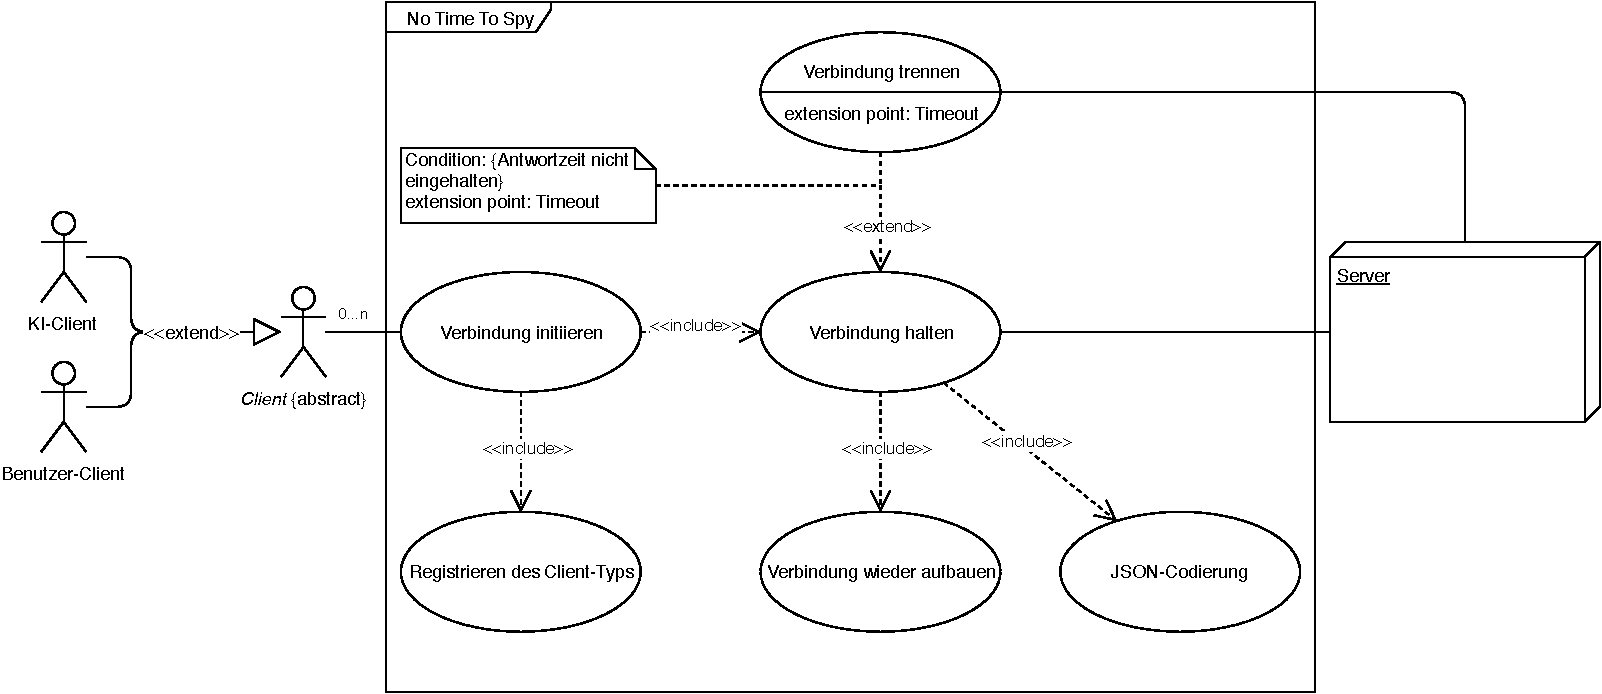
\includegraphics[width=\textwidth]{Meilenstein02/use_case_network.pdf}
  \caption{Anwendungsfälle Netzwerkverbindungsmanagement}
\end{figure}